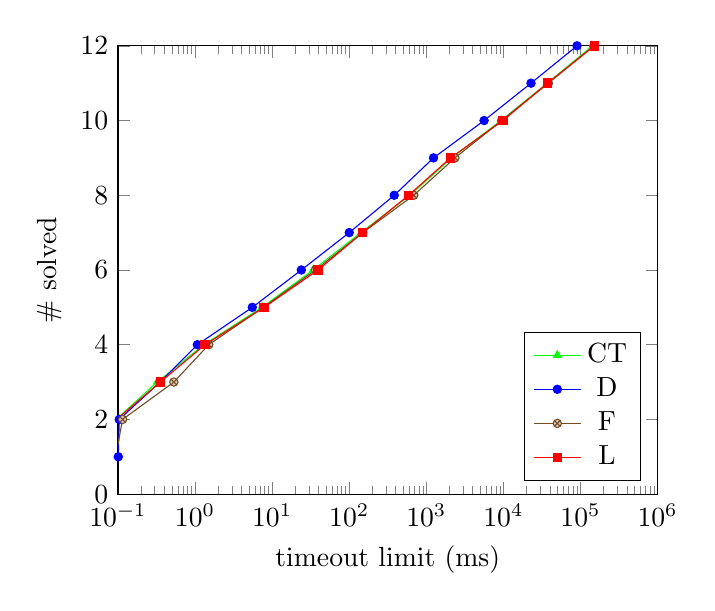
\begin{tikzpicture}[scale=1.0]
  \begin{axis}[
    xmode=log,
    ymin=0,ymax=12,
    xmin=0.1, xmax=1000000,
    every axis plot/.style={thin},
    xlabel={timeout limit (ms)},
    ylabel={\# solved},
    legend pos=south east
    % table/create on use/cumulative distribution/.style={
    %   create col/expr={\pgfmathaccuma + \thisrow{f(x)}}   
    % }
    ]
    \addplot 
    [mark=triangle*,
    mark size=1.5,
    mark options={solid},
    green] 
    coordinates {(0.092, 1)
(0.095, 2)
(0.323, 3)
(1.305, 4)
(7.407, 5)
(33.999, 6)
(142.189, 7)
(612.106, 8)
(2128.536, 9)
(9342.811, 10)
(37031.905, 11)
(143593.524, 12)};

    \addplot 
    [blue,
    mark=*,
    mark size=1.5,
    mark options={solid}]
    coordinates {(0.101, 1)
(0.104, 2)
(0.352, 3)
(1.072, 4)
(5.534, 5)
(23.943, 6)
(100.074, 7)
(383.914, 8)
(1238.844, 9)
(5618.200, 10)
(22809.152, 11)
(90056.907, 12)};

    \addplot [brown!60!black,
    mark options={fill=brown!40},
    mark=otimes*,
    mark size=1.5]
    coordinates {(0.093, 1)
(0.115, 2)
(0.531, 3)
(1.508, 4)
(7.667, 5)
(36.564, 6)
(150.260, 7)
(687.096, 8)
(2352.488, 9)
(9484.143, 10)
(38304.007, 11)
(149005.215, 12)};

    \addplot 
    [red,
    mark size=1.5,
    mark=square*]
    coordinates {(0.095, 1)
(0.096, 2)
(0.355, 3)
(1.348, 4)
(7.869, 5)
(39.453, 6)
(149.173, 7)
(590.206, 8)
(2064.396, 9)
(9858.869, 10)
(37441.670, 11)
(151868.885, 12)};
    \legend{CT,D,F,L}
  \end{axis}
\end{tikzpicture}
